C++中静态多态性的可用性,带来了实现经典设计模式的新方法。以桥接模式为例,在许多C++程序中扮演着重要的角色。使用桥接模式的一个目标是在接口的不同实现之间切换。

\begin{center}
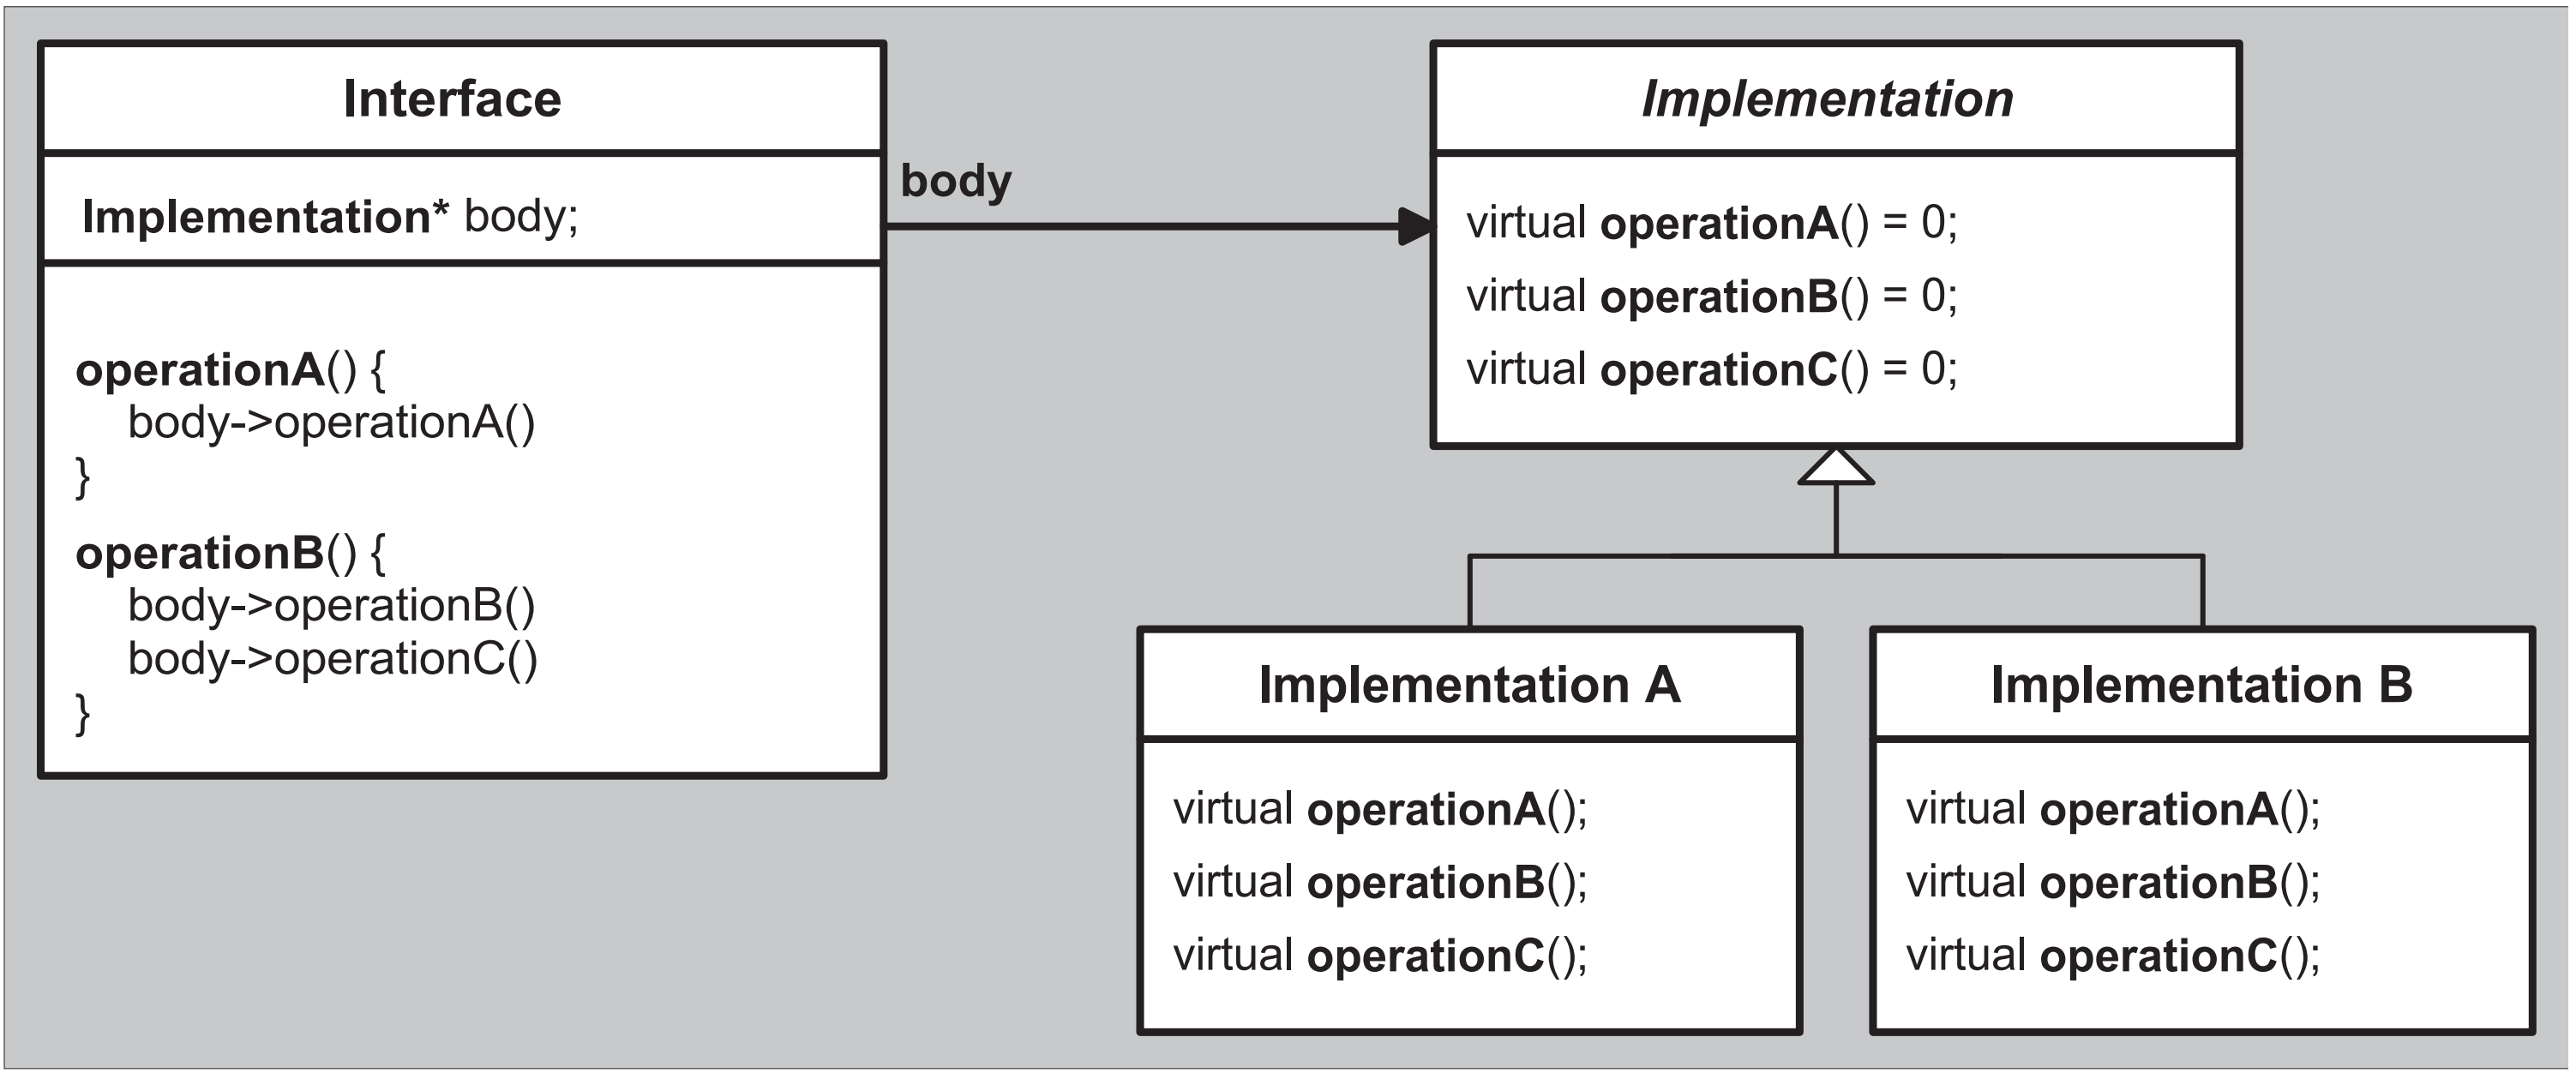
\includegraphics[width=0.8\textwidth]{content/3/chapter18/images/3.png} \\
图18.3. 使用继承实现的桥接模式
\end{center}

根据[DesignPatternsGoF],通过一个接口类来完成,嵌入一个指针来引用实际的实现,并通过这个指针委托所有调用(参见图18.3)。

但在编译时就知道实现的类型,那么可以利用模板的强大功能(参见图18.4),带来更好的类型安全性(部分原因是避免了指针转换)和性能。

\begin{center}
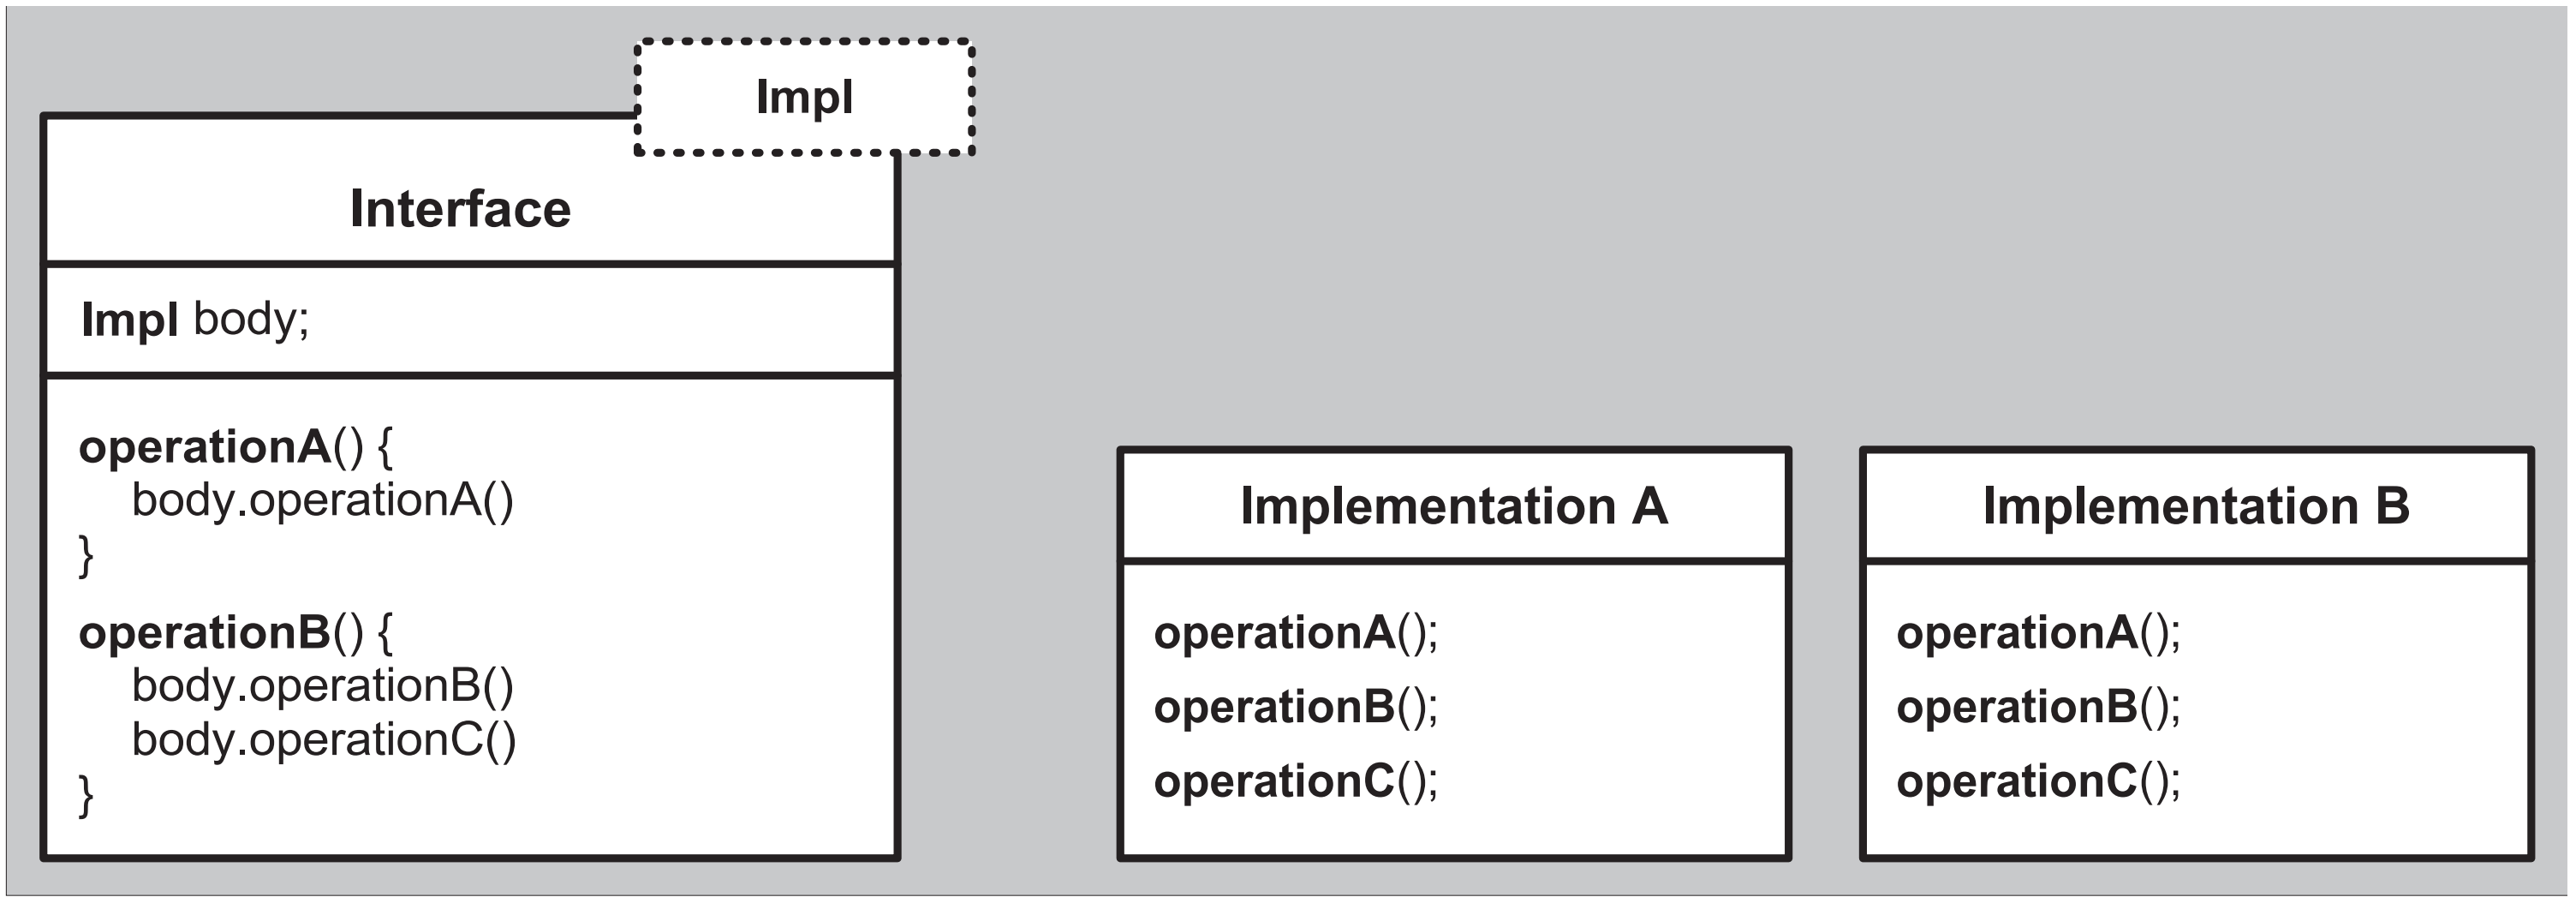
\includegraphics[width=0.8\textwidth]{content/3/chapter18/images/4.png} \\
图18.4. 使用模板实现的桥接模式
\end{center}










































